\documentclass{minimal}
\usepackage{tikz}
\usetikzlibrary{calc}
\begin{document}
	
	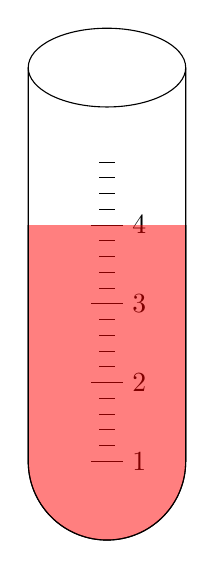
\begin{tikzpicture}
	\draw (0,0) ellipse (1 and .5);
	\draw (-1,0)--(-1,-5) arc (180:360:1)--(1,0);
	
	\foreach \y/\x in {-5/1,
		-4/2,
		-3/3,
		-2/4%
	}
	{
		\draw (-0.2,\y)--(0.2,\y) node[right](\x){\x};
		
		\foreach \z in {0.2,0.4,0.6,0.8}
		{\draw ($(-0.1,\z) + (0,\y)$)--($(0.1,\z)+(0,\y)$);}
	};
	
	\filldraw[fill opacity=0.5,fill=red](-1,-2)--(-1,-5) arc (180:360:1)--(1,-2);
	
	\end{tikzpicture}
	
\end{document}